\iffalse
%-*- program: xelatex -*-        
%-*- program: biber -*-`        
%-*- program: xelatex -*-
\documentclass[12pt]{article}
\usepackage{amsmath,textcomp,amssymb,geometry,graphicx,enumerate,upquote,color}
\usepackage{hyperref}
\usepackage{float}
\usepackage{breqn}
\usepackage{tikz}
\usepackage{array}
\usepackage{amsfonts}
\def\Session{Fall 2015}
\usepackage[english]{babel}
\title{Model Selection for the US Indices}
\author{Boying Gong, Xinyue Zhou}
\newenvironment{qparts}{\begin{enumerate}[{(}a{)}]}{\end{enumerate}}
\def\endproofmark{$\Box$}
\newenvironment{proof}{\par{\bf Proof}:}{\endproofmark\smallskip}
\begin{document}
\maketitle
\fi


\subsection{Introduction}
As described in the previous report, for financial assets, the returns have strong dependent across the time, thus it is reasonable to fit time series to interpret and predict them. In the study before,  the ARIMA model is used for fitting, while the diagnostics are infeasible for most assets. They cannot capture the variance cluster in the return, resulting in some variance cluster left the residual plot. In the example of RMZ  before, we are still able to fit at least one `'not too bad'' ARIMA model. However, for other assets, it almost impossible to fit arima: the autocorrelations are still there even after a long lag, and after we adding order more than p = 5, q = 5, the convergence issue always happens. However, we still attach the best ARIMA for each assets we can find to the end.

In this report, we search to apply another widely used model, GARCH,  to fit the returns, and also catch the variance clusters in the them. It turns out to have a much better performance in capturing the variance, and the diagnostic are also showing a delightful patterns

\subsection{Diagnostics of ARMA}
Under our context, Garch models are mainly used for clustered residual left in ARMA model. Therefore, to ensure that GARCH is in need, normally, one should first plot the residuals and other diagnostics of the existing ARMA model. Then from the diagnostics, conclusion can be made if GARCH is necessary and what are the GARCH parameters.

The follow plot is an example of RMZ assets. In the previous study, we found the best ARIMA model for RMZ is MA(1), the diagnostic plot is attached below. Again, the variance clusters in the residual are not captured in the model.

\begin{figure}
  \caption{Diagnostic Plots of MA(1) for RMZ}
  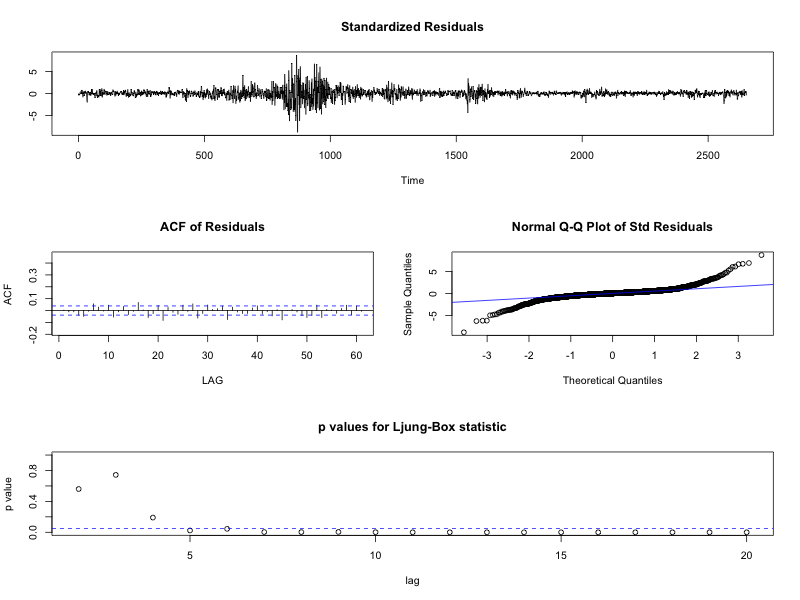
\includegraphics[width = \textwidth]{../results/DiagnosticRMZ}
  \label{fig:DiagnosticRMZ}
\end{figure}

In all the ten American indices, except for \textbf{G0O1}, it is the common phenomenon that assets have the clustered variance, and thus, the GARCH model is in need for model the residuals, as is shown in the Figure \ref{fig:DiagnosticResids}.

\begin{figure}
  \caption{Residuals after fitting using the best ARIMA Model}
  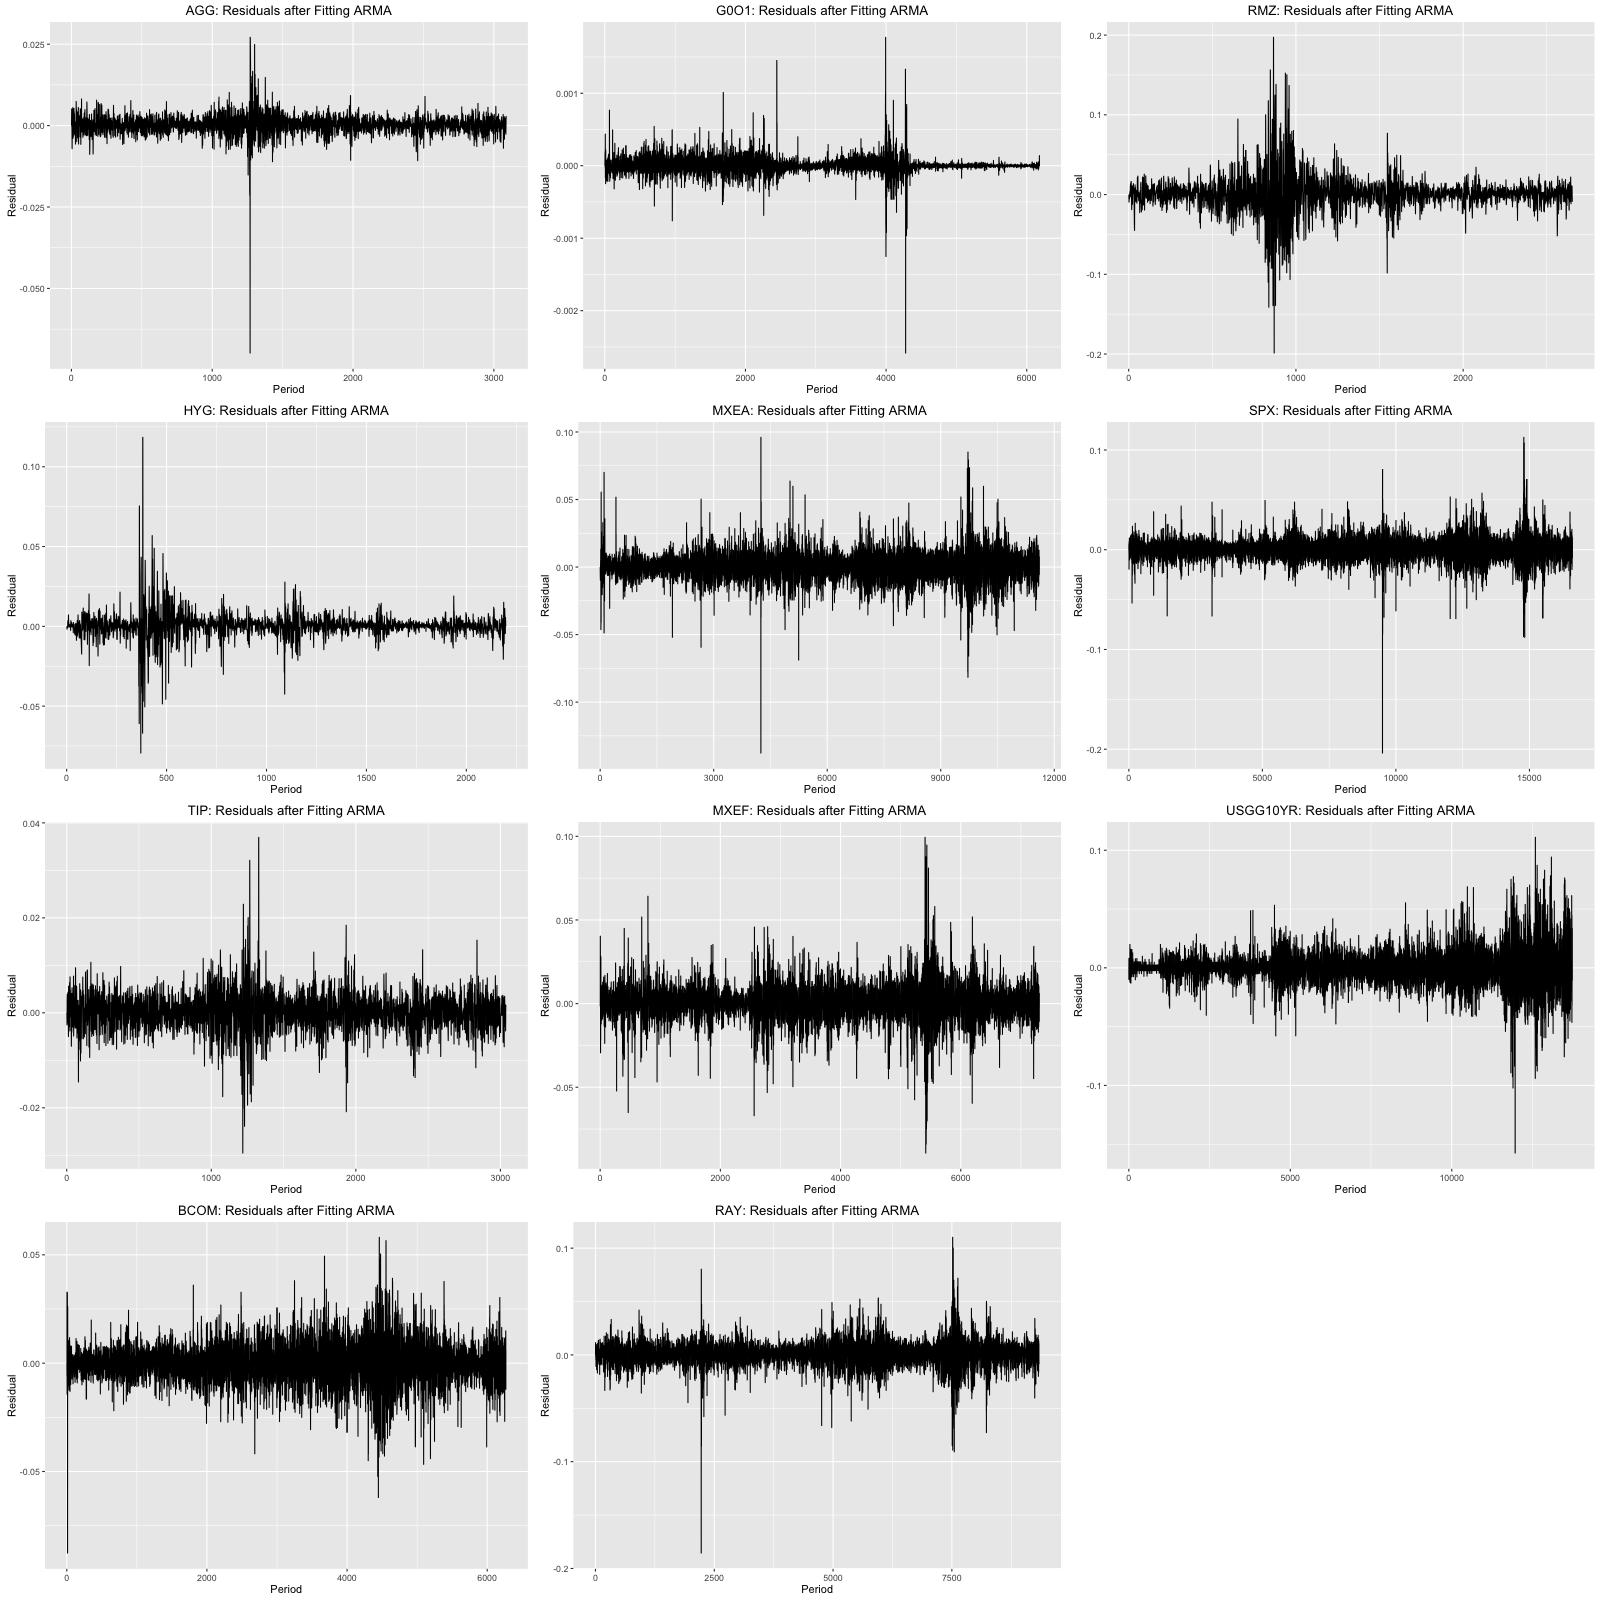
\includegraphics[width = \textwidth]{../results/resids}
  \label{fig:DiagnosticResids}
\end{figure}

The Table \ref{table:BestArima} shows the `'best'' ARIMA model selected from a set of ARIMA parameters. Noticing that model for G0O1is ignored from the analysis, since G0O1 is too stable and always used for free-risk rate.

\begin{table}[!h]
\caption{Best ARIMA Model for the U.S. Assets }
\centering 
\begin{tabular}{ | c || r | } 
 \hline
Asset & ARIMA (p,d,q) \\
  \hline \hline
AGG & (5,0,5) \\ 
HYG & (3,0,1) \\ 
TIP &  (0,0,0)\\ 
BCOM & (0,0,0)\\ 
MXEA & (2,0,2) \\ 
MXEF & (4,0,2)\\ 
RAY &  (2,0,2)\\ 
RMZ & (0,0,1) \\ 
SPX & (2,0,2) \\ 
USGG10YR & (0,0,0) \\
 \hline
\end{tabular}
\label{table:BestArima}
\end{table}

\subsection{Fit Garch Model}
In this section,  RMZ is chosen as an example to explain the process of fitting GARCH, and corresponding diagnostics. RMZ is selected to continue the study in the previous report. RMZ, as shown before, is selected considering its short period, larger series correlaitions, larger risk measurements, and less mode in the Maximum Draw Down.

GARCH(1,1) is the most widely used the model in financial assets, so we fit the residual in MA(1) to GARCH(1,1) here. Rather than ARIMA having constant variance assumption, GARCH(1,1) also model the heteroscedasiticity in the time series.  For GARCH(1,1), the model is discribed as following:

\begin{align*}
y_t & = \sigma_t \epsilon_t\\
\sigma_t^2 & = \alpha_0+ \alpha_1 y_{t-1}^2 +\beta_1\sigma_{t-1}^2
\end{align*}


The residuals left after modeling ARIMA are extracted to feed to GARCH model. The range of GARCH parameters are always hard to figure out just from the plots of diagnostic, so a set GARCH models are applied to each real data. Then we chose the best model based on the BIC criterion. The reason why BIC is used instead of AIC or AICc is that BIC always penalize more on extra parameters and suggest a smaller model, avoiding the overfitting problem.

After fitting the GARCH models on the residuals left from ARMA models, diagnostics are conducted on each GARCH model. It is a common situation that all the autocorrelations between residuals have been highly reduced after modeling, which mean GARCH effectively model the residuals. The Table \ref{table:BestGarch} present the best GARCH model according to BIC values. 

\begin{table}[!h]
\caption{Best GARCH Model for the residuals after Fitting ARIMA}
\centering 
\begin{tabular}{ | c || r | } 
 \hline
Asset & ARIMA (p,q)+ GARCH(m,n) \\
  \hline \hline
AGG & ARMA(5,5)+GARCH(1,1) \\ 
HYG & ARMA(3,1)+GARCH(1,1) \\ 
TIP &  GARCH(1,1)\\ 
BCOM & GARCH(1,1)\\ 
MXEA & ARMA(2,2)+ GARCH(1,2) \\ 
MXEF & ARMA(4,2) + GARCH(1,1)\\ 
RAY &  ARMA(2,2) + GARCH(1,1)\\ 
RMZ & MA(1) + GARCH(1,1) \\ 
SPX & ARMA(2,2) +GARCH(1,1)\\ 
USGG10YR & GARCH(1,3) \\
 \hline
\end{tabular}
\label{table:BestGarch}
\end{table}


 We are also faced with several problems in diagnostics, after finding the most reasonable GARCH parameters. The first thing needs to be mentioned is that it always appears heavy tail problem after fitting.  The residual left after GARCH is almost white noise  , which is a good sign for eliminating the correlations between points, as ACF plots. However, the heavy tail is existing as the sign from the normal Q-Q plots   , in which points deviate from line at both ends. Several approach can be adopted to fix heavy tail, one of which is that instead of normal, using Student t distribution as conditional distribution in the GARCH. Alternatively, Generalize Normal Distribution (GED) can also used as conditional distribution to somehow alleviate heavy tail. QMLE is another potential option. 
 
 The other concern we meet in the analysis is that, even though after fitting GARCH, some of the autocorrelation still left in the residuals, and it more commonly happens on the first order correlation. Several derivative class of GARCH model are specifically used for handle this problem, while we left it for future analysis, as it does no harm for our prime research.


\subsubsection{An Example: RMZ}
In the previous study, we found the best ARIMA model for RMZ is MA(1), the diagnostic plot is attached below. Again, the variance clusters in the residual are not captured in the model.

\begin{figure}
  \caption{Diagnostic Plots of MA(1) for RMZ}
  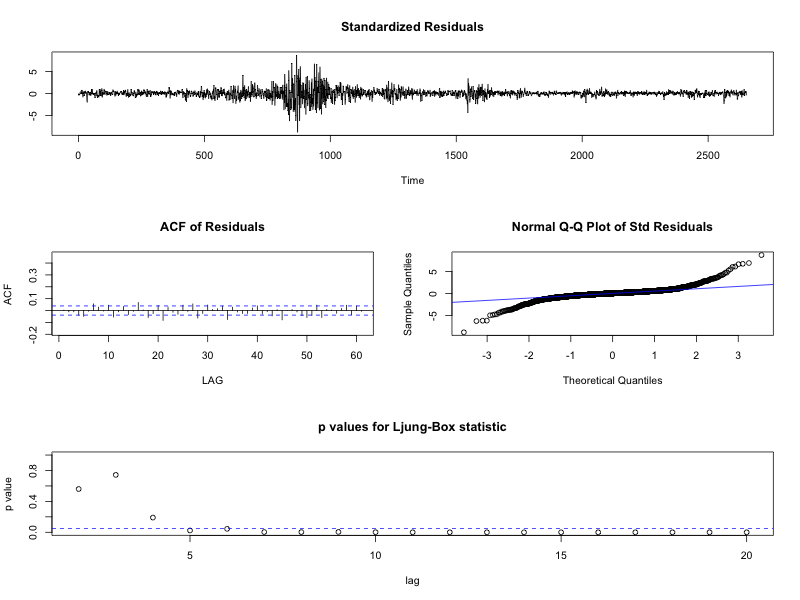
\includegraphics[width = \textwidth]{../results/DiagnosticRMZ}
  \label{fig:DiagnosticRMZ}
\end{figure}

Fit the residual of MA(1) to GARCH(1,1), we got the follow model:
\begin{align*}
R_t &= -4.1561\times 10^{-2}\epsilon_{t-1} \\
\sigma_t^2 & = 1.9955 \times 10^{-6} +1.1083\times 10^{-1} T_{t-1}^2 +8.8506\times 10^{-1}  \sigma_{t-1}^2
\end{align*}

The Figure \ref{fig:RMZ_GARCH_dig1} are the plots of the standardized residuals. 

\begin{figure}
  \caption{RMZ: Diagnostic Plots of GARCH(1,1) with Gaussian Conditonal Distribution}
  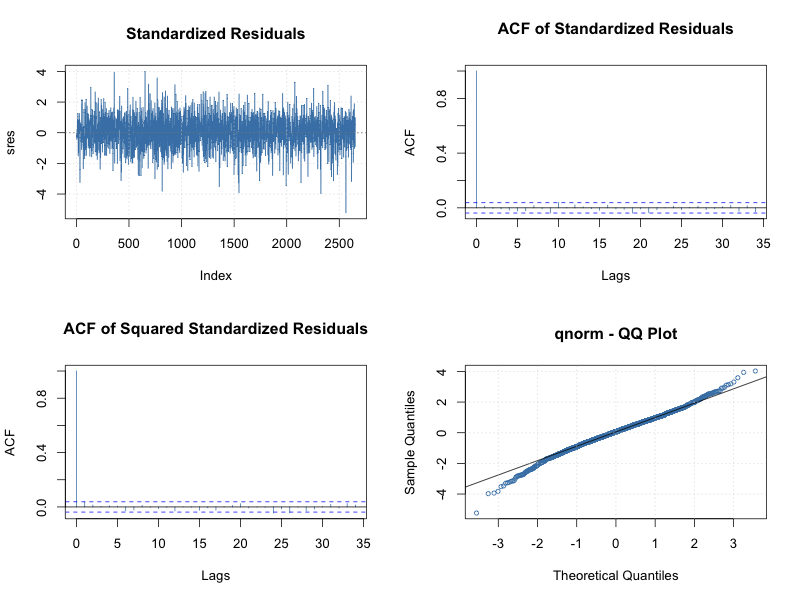
\includegraphics[width = \textwidth]{../results/RMZ_GARCH_dig1}
  \label{fig:RMZ_GARCH_dig1}
\end{figure}

After fitting GARCH, the residual left is almost white noise, which is a good sign for eliminating the correlations between points, as evidented in the next two ACF plots. However, the heavy tail problem is still there. Several approach can be adopted to fix it, one of which is instead of normal, using Student t distribution as conditional distribution in the GARCH. Finding t distribution is not really solve the problem, we finally chose to use Generalize Normal Distribution (GED) as the conditional distribution. QMLE is another potential alternative. The Figure \ref{fig:RMZ_GARCH_dig2} indicates that the heavy tail problem is almost solved in the by applying GED.

\begin{figure}
  \caption{RMZ: Diagnostic Plots of GARCH(1,1) with GED Conditonal Distribution}
  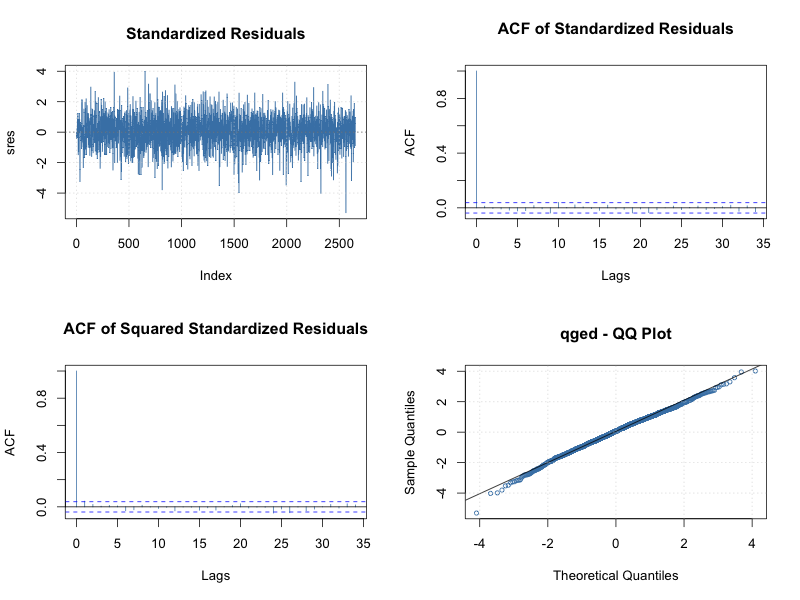
\includegraphics[width = \textwidth]{../results/RMZ_GARCH_dig2}
  \label{fig:RMZ_GARCH_dig2}
\end{figure}

Figure \ref{fig:RMZ_GARCH_ESTsd} the plot compare the estimation of standard deviation using GARCH(1,1), with using naive estimate of standard deviation. The black continuous line is the estimate of the instantaneous conditional standard deviation of the GARCH(1,1). The large peak indicative of the huge standard deviation corresponding to the crisis of 2008. Red line is the empirical standard deviation of the entries of the series in the window containing the entries of the last 30 days.  As shown in the plot, the naive estimator is smoother than GARCH, while they almost follow the sample trend.
\begin{figure}
  \caption{RMZ: Estimate of the Instantaneous Conditional Standard Deviation}
  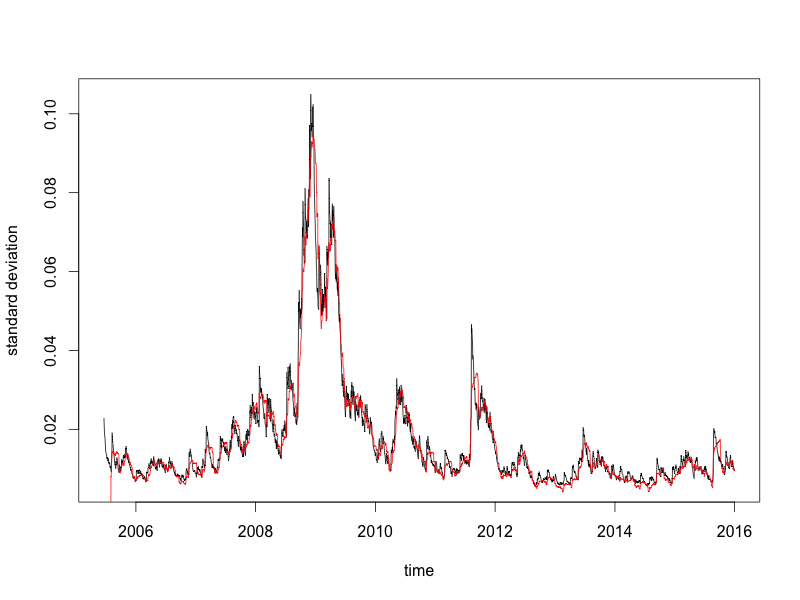
\includegraphics[width = \textwidth]{../results/RMZ_GARCH_ESTsd}
  \label{fig:RMZ_GARCH_ESTsd}
\end{figure}

Figure \ref{fig:RMZ_GARCH_predCI} show the last 120 residuals from MA(1), we used all but last 20 to fit the GARCH(1,1) model with GED conditional distribution and create an confident interval based on that. And it is nice to see that all the last 20 points lies in the interval.

\begin{figure}
  \caption{RMZ: Estimate of the Instantaneous Conditional Standard Deviation}
  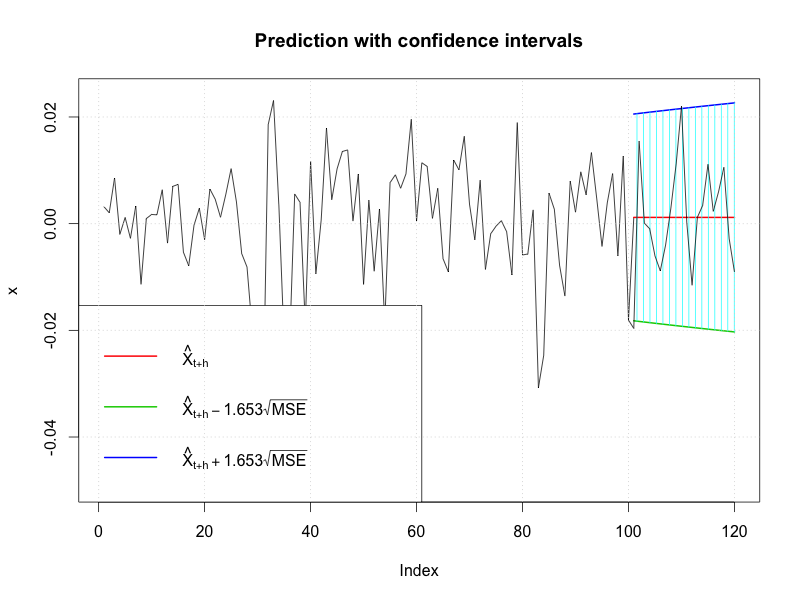
\includegraphics[width = \textwidth]{../results/RMZ_GARCH_predCI}
  \label{fig:RMZ_GARCH_predCI}
\end{figure}

In summary, instead of assuming constant variance using ARIMA, modeling the residuals from MA(1) using GARCH(1,1) seems to be more reasonable for RMZ.

\subsubsection{Summary of Results}
This section answer the questions that what kind of model should be selected for modeling the return of financial assets. Model selection hints from the descriptive statistics are also highlighted. It gives people an intuition and helps to narrow down the potential parameter sets, and thus reduce the work load. However, this is not the general rule. In order to decide the most suitable model, one should take a close look at the time series properties and compare several possible models using model selection criterions.

\begin{itemize}
\item Essentially, ARMA component do not need to be there. For those time series, conditional means are almost fixed, such as TIP, BCOM and USGG10YR. Some of statistics are able to indicate this on some extent. For example, a very high Sharpe Ratio, meaning the low return and high standard deviation, suggests that it is hard for using ARIMA  to capture the change of conditional mean in too much noise. Moreover, based on study, we found that the returns of assets with smaller absolute skewness values are more likely free from ARMA component. As can be imagined, if an asset is high skewed, it is a highly possible situation that the returns deviate from mean value at some certain time period because of economics events.
\item ARMA component sometimes is just not enough to characterize the timeseries, indicated a unstationary residuals even after a long lag. Based on my experience, the trial until p =5 and q = 5 is adequately detection for ARMA component. The change of model or adding GARCH component should be taken into consideration when larger lags in need.
 \item For the financial essets we already took a close look at, the GARCH model is always required, as the evidenced by the clustered variance in the return. Financial assets tend to have higher or lower volatility in a certain period as the result of some economics events, such as a higher fluctuation around 2008 crisis.
  \item GARCH(1,1) are always enough for charaterize the clustered variance in financial assets. Even though I select GARCH(1,2) and GARCH(1,3) for MXEA and USGG10YR based on BIC, GARCH(1,1) still works good for these two indices, showing almost no differents in diagnostic plots. 
\end{itemize}


Next present the model for each index. Those are from analysis that repeat over and over again in the previous section. To avoid redundancy, the full analysis is not showing out. The stars in the equations below represents the significance level of the coefficents. 


\begin{enumerate}
\item \textbf{AGG} (BIC = -6.8688):
\begin{dmath*}
R_t  = -0.0698R_{t-1} + 0.5235R_{t-2} - 0.7308R_{t-3}- 0.4478 R_{t-4}
+0.5656 R_{t-5} -0.0771 \epsilon_{t-1}  -0.5810\epsilon_{t-2} 
+0.774\epsilon_{t-3} +0.3736\times 10^{-4}\epsilon_{t-4}  -0.6190 \epsilon_{t-5} 
\end{dmath*}
\begin{align*}
\sigma_t^2  = 9.3294 \times 10^{-8} +6.8088\times 10^{-2} T_{t-1}^2(^{***}) +9.1898\times 10^{-1}  \sigma_{t-1}^2(^{***})\\
\end{align*}


\item \textbf{HYG} (BIC = -6.8688):
\begin{dmath*}
R_t = -0.5756R_{t-1} -0.0207R_{t-2}  -0.0996R_{t-3}
+ 0.5775 \epsilon_{t-1} 
\end{dmath*}
\begin{align*}
\sigma_t^2  &= 4.312 \times 10^{-7} +1.712\times 10^{-1} T_{t-1}^2(^{***}) +8.467\times 10^{-1}  \sigma_{t-1}^2(^{***})\\
\end{align*}

\item \textbf{TIP} (BIC = -8.3838):
\begin{align*}
\sigma_t^2  &= 1.752 \times 10^{-7} +5.254\times 10^{-2} T_{t-1}^2(^{***}) +9.357e\times 10^{-1}  \sigma_{t-1}^2(^{***})\\
\end{align*}


\item \textbf{BCOM} (BIC =-6.7632):
\begin{align*}
\sigma_t^2  &= 2.640 \times 10^{-7} +4.536\times 10^{-2} T_{t-1}^2(^{***}) +9.523e\times 10^{-1}  \sigma_{t-1}^2(^{***})\\
\end{align*}

\item \textbf{MXEA} (BIC = -6.7857):
\begin{dmath*}
R_t = -0.2176R_{t-1} -0.4230R_{t-2} 
 0.3240\epsilon_{t-1} + 0.4305 \epsilon_{t-2} + 0.0248 \epsilon_{t-3} +  0.0394 \epsilon_{t-4} 
\end{dmath*}
\begin{dmath*}
\sigma_t^2  = 1.1415\times 10^{-6} +1.2141\times 10^{-1} T_{t-1}^2(^{***}) +5.1514\times 10^{-1}  \sigma_{t-1}^2(^{***}) +3.5499\times 10^{-1}  \sigma_{t-2}^2(^{***})\\
\end{dmath*}


\item \textbf{MXEF} (BIC =-6.5399):
\begin{dmath*}
R_t = -0.6328R_{t-1}+  0.1588R_{t-2} -0.0038R_{t-3}  -0.0093R_{t-4} +
 0.8807\epsilon_{t-1} +  0.0279 \epsilon_{t-2} 
\end{dmath*}
\begin{dmath*}
\sigma_t^2  = 1.4479\times 10^{-6} + 9.8248\times 10^{-2} T_{t-1}^2(^{***}) +8.9191\times 10^{-1}  \sigma_{t-1}^2(^{***}) \\
\end{dmath*}


\item \textbf{RAY} (BIC =-6.6313):
\begin{dmath*}
R_t = 0.2526R_{t-1}+  0.3255R_{t-2} -0.2553\epsilon_{t-1} -0.3649 \epsilon_{t-2} 
\end{dmath*}
\begin{dmath*}
\sigma_t^2  = 1.1770\times 10^{-6} + 7.2784\times 10^{-2} T_{t-1}^2(^{***}) +9.1646\times 10^{-1}  \sigma_{t-1}^2(^{***}) \\
\end{dmath*}


\item \textbf{RMZ} (BIC =-5.6962):
\begin{dmath*}
R_t = -4.1561\times 10^{-2}\epsilon_{t-1} 
\end{dmath*}
\begin{dmath*}
\sigma_t^2  = 1.9955 \times 10^{-6} +1.1083\times 10^{-1} T_{t-1}^2(^{***})  +8.8506\times 10^{-1}  \sigma_{t-1}^2(^{***}) 
\end{dmath*}

\item \textbf{SPX} (BIC =-6.8697):
\begin{dmath*}
R_t =  0.3488R_{t-1}+  0.2556R_{t-2}  -0.3185\epsilon_{t-1}  -0.3083\epsilon_{t-2} 
\end{dmath*}
\begin{dmath*}
\sigma_t^2  = 6.39\times 10^{-7} + 7.4752\times 10^{-2} T_{t-1}^2(^{***}) +9.1971\times 10^{-1}  \sigma_{t-1}^2(^{***}) \\
\end{dmath*}


\item \textbf{USGG10YR} (BIC = -6.664873):
\begin{dmath*}
\sigma_t^2  = 1.1789 \times 10^{-8} +1.0817\times 10^{-1} T_{t-1}^2 (^{***}) +5.10\times 10^{-1}  \sigma_{t-1}^2(^{***}) 
+10^{-8}  \sigma_{t-2}^2(^{***}) 
+3.9287\times 10^{-1}  \sigma_{t-3}^2(^{***}) 
\end{dmath*}
\end{enumerate}

\subsection{Serial Correlation and Risk Measurement}
After the model selection, we now can check the relationship between serial correlations and risk measurements using the best model we get. Finding sometimes it meets some converging problem when apply the best model on subset of the data, I some times also use the second best model. For this reason, instead of  using ARMA(2,4) for MXEA, ARMA(4,2) for MXEF and (2,2) for SPX, I used MA(2) for MXEA,  AR(3) for MXEF and MA(2) for SPX. Table \ref{table:vsRiskMeasure} directly gives the correlation coefficents between first-order serial correlation and risk measurements.

It shows that it generally has a negative relationship between serial correlation and risk measurements. Some of them are quite small, such as MXEF, -0.0379 for VaR even after using the best model. Some of them are comparatively high, such as RMZ, as high as 0.8621 for VaR.

 Generally speaking,  relationship between between first-order serial correlation and risk measurements are very close. $\rho$'s with CED are always smaller than that with other risk measurements, considering the absolute value .Table\ref{table:vsRiskMeasure} also suggests that CED is not necessary to be negative. However, we find that for CED positively related to serial correlation, the corresponding $\rho$ with VaR or ES are also very small, though negative. 


\begin{figure}
  \caption{Relationship First-order Serial Correlation and VaR using Best Model}
  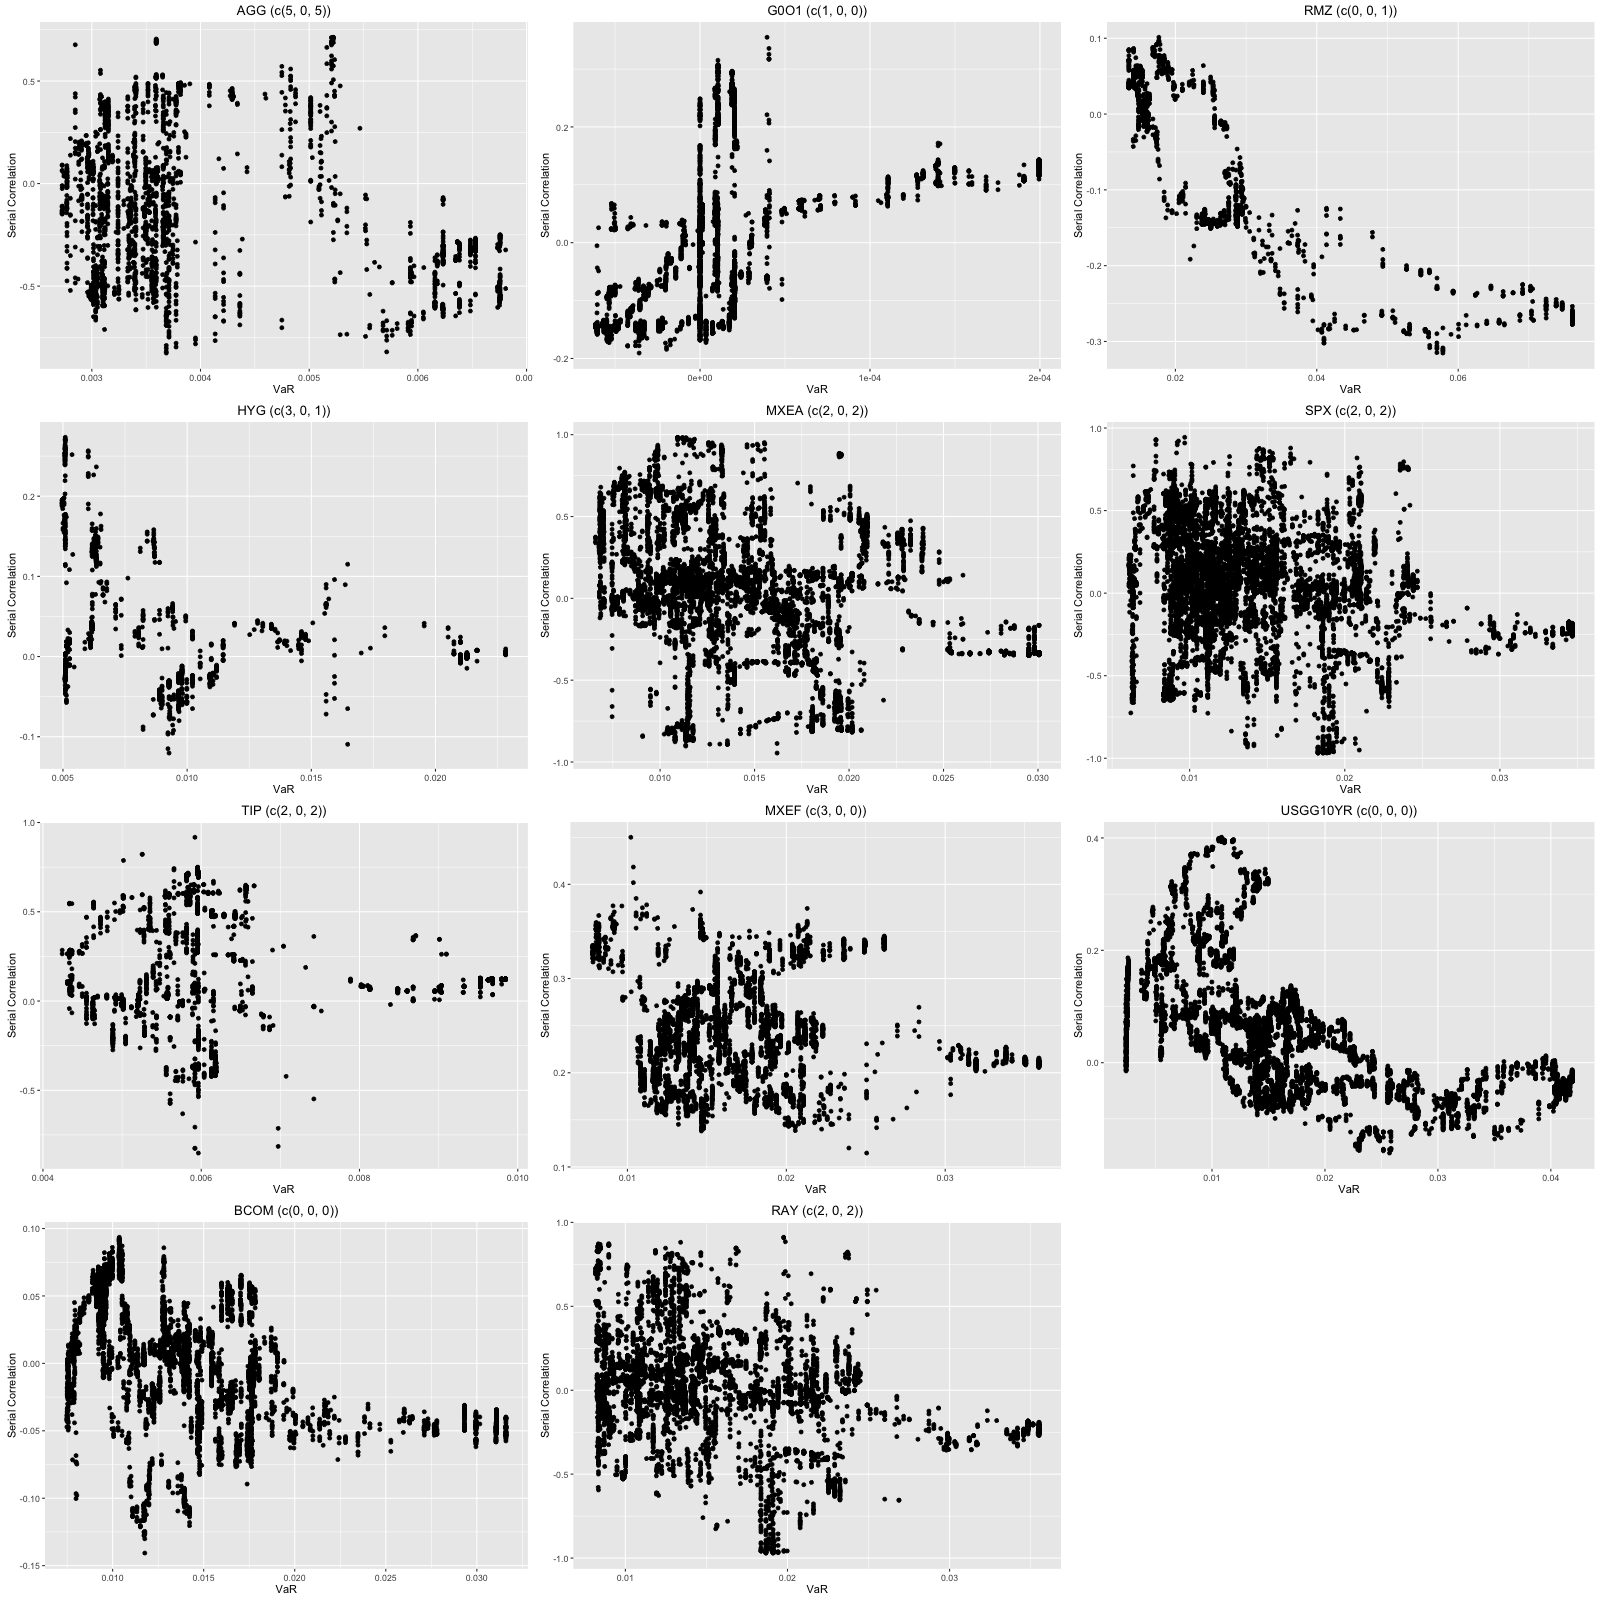
\includegraphics[width = \textwidth]{../figures/SerCol-VaR2yr}
  \label{fig:SerCol-VaR2yr}
\end{figure}

\begin{figure}
  \caption{Relationship First-order Serial Correlation and ES using Best Model}
  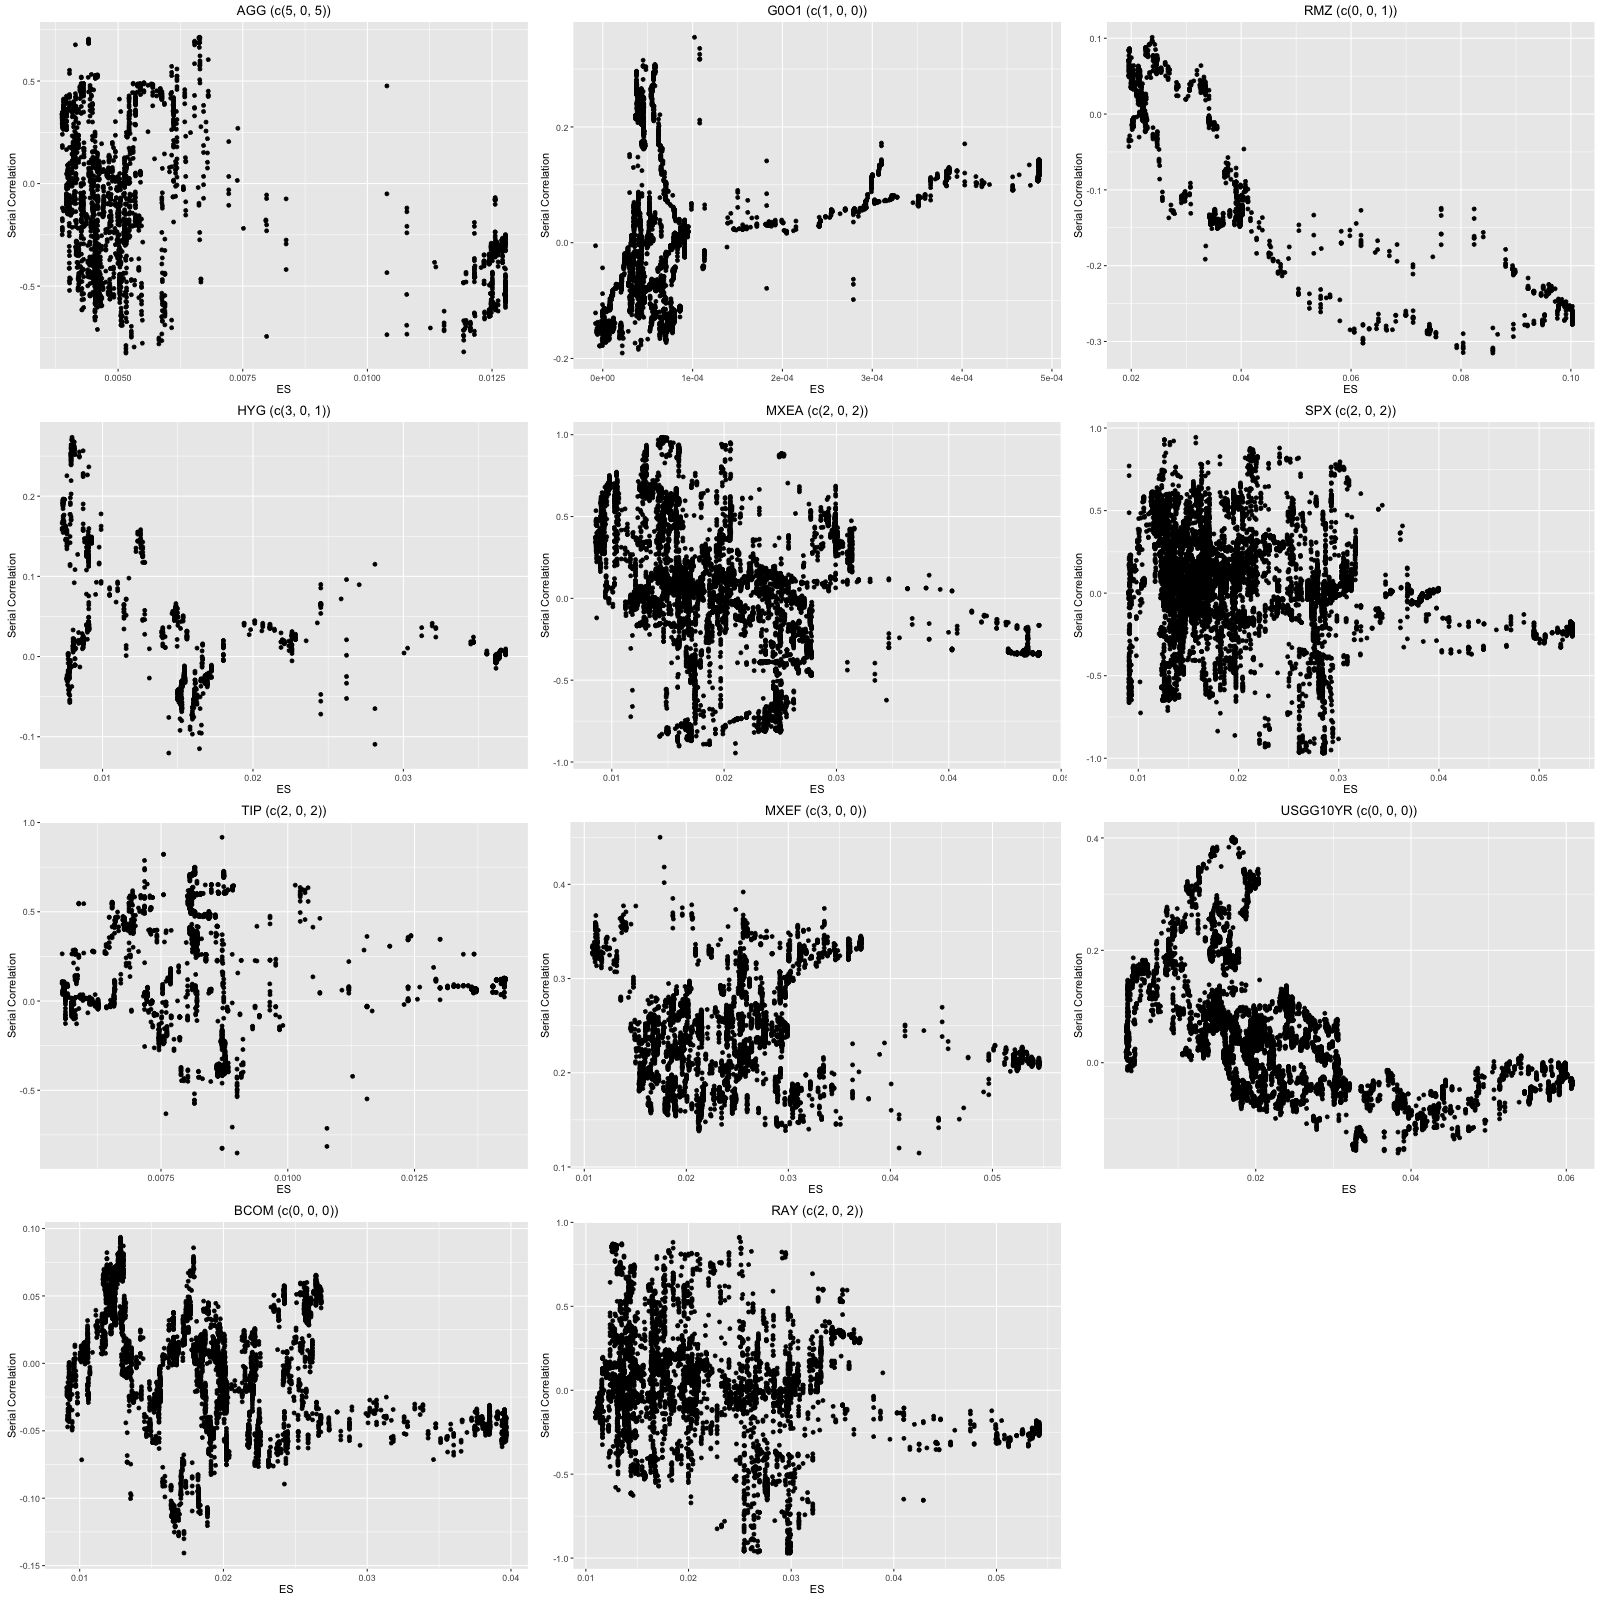
\includegraphics[width = \textwidth]{../figures/SerCol-ES2yr}
  \label{fig:SerCol-ES2yr}
\end{figure}

\begin{figure}
  \caption{Relationship First-order Serial Correlation and CED using Best Model}
  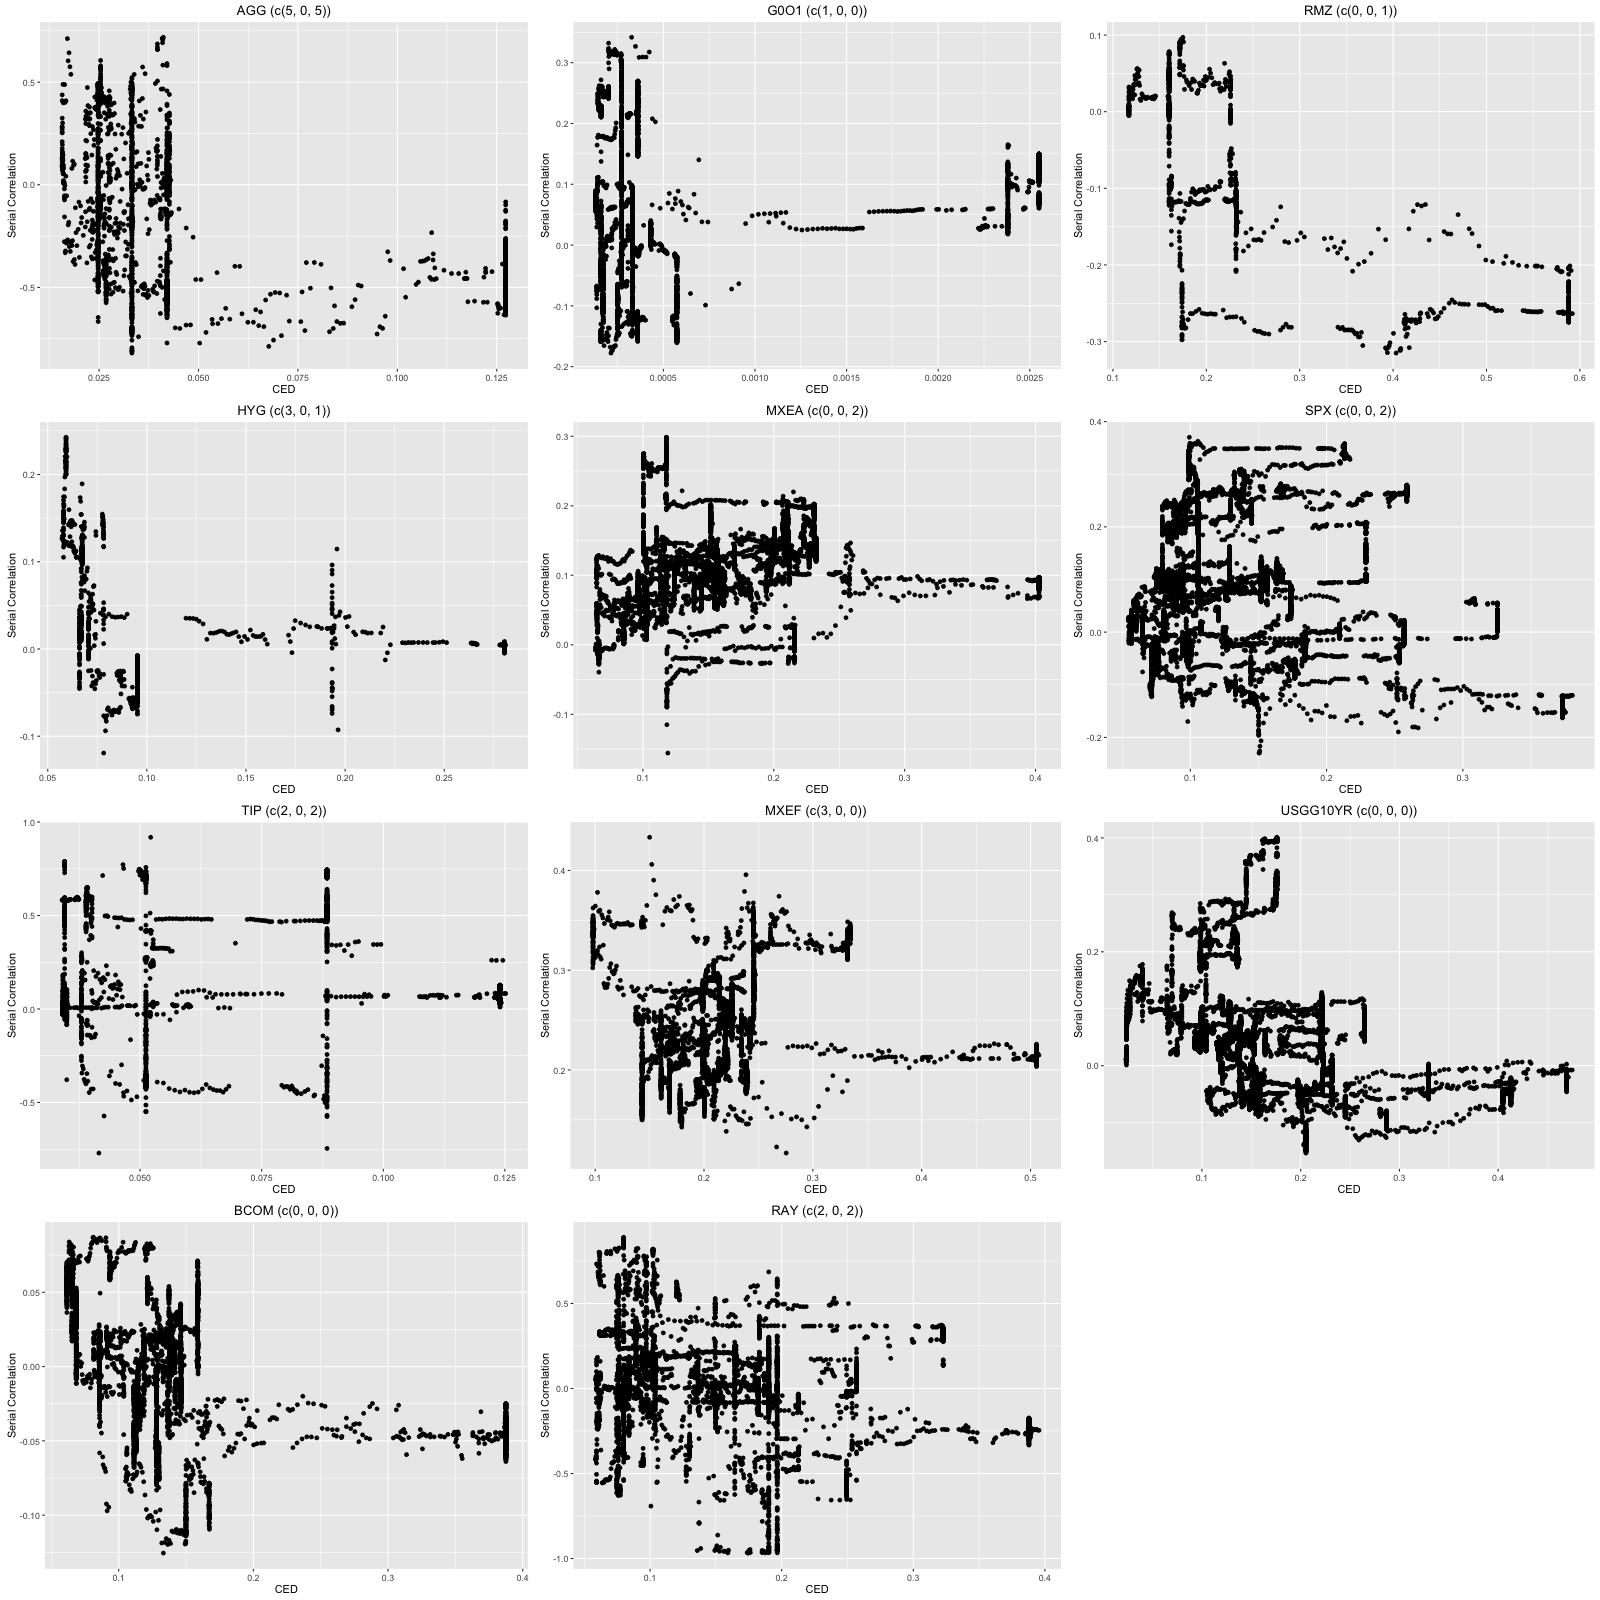
\includegraphics[width = \textwidth]{../figures/SerCol-CED3mon2yr}
  \label{fig:SerCol-CED3mon2yr}
\end{figure}

\begin{table}[!h]
\caption{Correlation between First-order Serial Correlation and Risk Measurements}
\centering 
\begin{tabular}{ | c || r | r | r | r |} 
 \hline
Asset& Model & v.s. VaR & v.s. VaR &v.s. CED\\
  \hline \hline
AGG &ARMA(5,5) &-0.2456 &  -0.3605&-0.3972 \\ 
HYG &ARMA(3,1) & -0.3162& -0.3346 & -0.2419 \\ 
TIP & AR(1)  &-0.0369 & -0.0660 & 0.0286 \\ 
BCOM &AR(1) & -0.4291&  -0.3897& -0.4298\\ 
MXEA & MA(2) &-0.3358&  -0.3542& 0.1402\\ 
MXEF & AR(3)  &-0.0379  &  -0.0084& 0.0958\\ 
RAY & MA(1) &-0.3459 &   -0.2611&  -0.2234\\ 
RMZ & ARMA(2,2) &-0.8621 &  -0.8763&  -0.7949\\ 
SPX & MA(2)  &-0.1983 &  -0.2267& -0.1220\\ 
USGG10YR &  AR(1) &-0.5578&  -0.5168& -0.3866\\
 \hline
\end{tabular}
\label{table:vsRiskMeasure}
\end{table}

\subsection{A Small Simulation Study}
We simulated a AR(1) time series and want to take a look at the relationship between risk measurements and serial correlations. The Figure \ref{fig:SimPart2} shows that VaR/ES has a positive relationship with first-order serial correlation. This is strange compared with the conclusion we have got in the previous section, which is in need of deeper analysis.
\begin{figure}
  \caption{Sim AR(1): First-order Serial Correlation and Risk Measurements}
  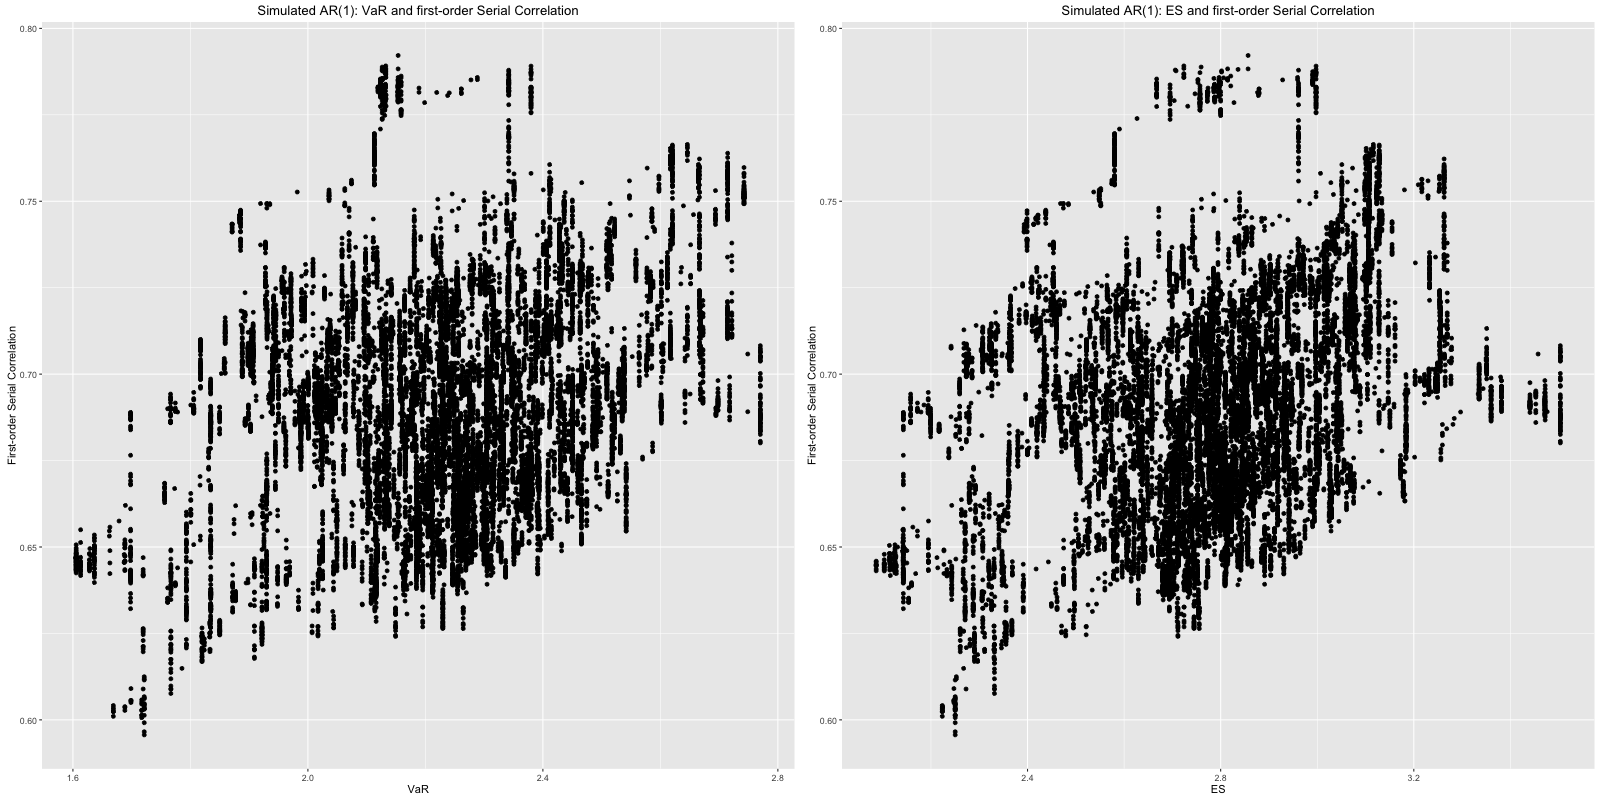
\includegraphics[width = \textwidth]{../figures/sim_part2}
  \label{fig:SimPart2}
\end{figure}
%\end{document}
